\documentclass[11pt]{report}
\usepackage[letterpaper, total={6.5in, 10in}]{geometry}
%\usepackage{fancyhdr}
%\pagestyle{fancy}
\usepackage{amsmath, amsthm, mathpazo, epic, eepic, color, array}
\usepackage{amssymb}
%\usepackage{graphicx}
\usepackage{cancel}
\usepackage{pgfplots}
\usepackage{multicol}
\pgfplotsset{compat=1.13}
\usepackage{etoolbox}
\makeatletter
\patchcmd{\chapter}{\if@openright\cleardoublepage\else\clearpage\fi}{}{}{}
\makeatother
\usepackage{hyperref}

\usepackage{enumerate}
\usepackage{enumitem}

\usepackage{tikz}
\usetikzlibrary{positioning,chains,fit,shapes,calc,arrows,patterns}
\usepackage{tkz-graph}
\usetikzlibrary{arrows, petri, topaths}
\usepackage{tkz-berge}
\usepackage[all]{xy}
\usepackage{textcomp}

\newboolean{colorprint}
\setboolean{colorprint}{true}
%\setboolean{colorprint}{false}

\ifthenelse{\boolean{colorprint}}{%
\newcommand{\colorone}{blue}
\newcommand{\colortwo}{red}
\newcommand{\coloronefill}{blue!15!white}
\newcommand{\colortwofill}{red!15!white}
\newcommand{\colormapone}{rgb=(.4,.4,1); rgb=(.8,.8,1)}
\newcommand{\colormaptwo}{rgb=(1,.4,.4); rgb=(1,.8,.8)}
\newcommand{\colormapplaneone}{rgb=(.7,.7,1); rgb=(.9,.9,1)}
\definecolor{colormaponebottom}{rgb}{.4,.4,1}
\definecolor{colormaponetop}{rgb}{.8,.8,1}
\definecolor{colormaptwobottom}{rgb}{1,.4,.4}
\definecolor{colormaptwotop}{rgb}{1,.8,.8}
}% ends color
{% not color
\newcommand{\colorone}{black}
\newcommand{\colortwo}{black!50!white}
\newcommand{\coloronefill}{black!15!white}
\newcommand{\colortwofill}{black!05!white}
\newcommand{\colormapone}{rgb=(.4,.4,.4); rgb=(.7,.7,.7)}
\newcommand{\colormaptwo}{rgb=(.6,.6,.6); rgb=(.9,.9,.9)}
\newcommand{\colormapplaneone}{rgb=(.8,.8,.8); rgb=(.95,.95,.95)}
\definecolor{colormaponebottom}{rgb}{.4,.4,.4}
\definecolor{colormaponetop}{rgb}{.7,.7,.7}
\definecolor{colormaptwobottom}{rgb}{.6,.6,.6}
\definecolor{colormaptwotop}{rgb}{.9,.9,.9}
}%

\newlength\tindent
\setlength{\tindent}{\parindent}
\setlength{\parindent}{0pt}
\renewcommand{\indent}{\hspace*{\tindent}}

\pgfplotsset{my style/.append style={axis x line=middle, axis y line=
middle, xlabel={$x$}, ylabel={$y$}, axis equal }}

\pgfplotsset{compat=1.13}
\newcommand{\ds}{\displaystyle}
\begin{document}


\textbf{4.2 Additional Example}\\
\vskip .5 truecm

\textbf{Example 4.2.4 Optimization: Minimizing Surface Area}\\
Design a closed cylindrical can of volume $8$ ft$^3$ so that it uses the least amount of metal. In other words, minimize the surface area of the can.\\

%I stole this picture from somewhere else and I can't figure out how to make it smaller!!!%%%
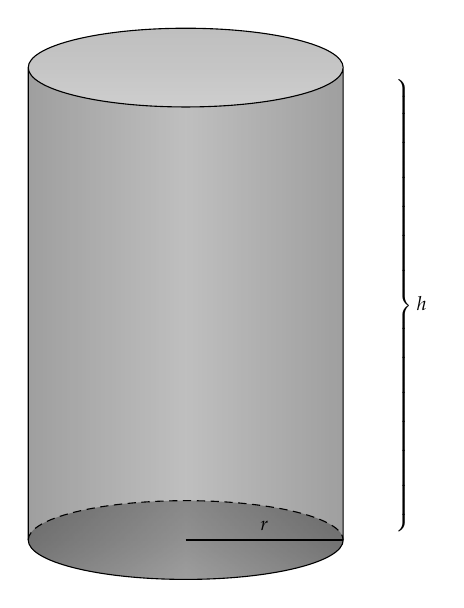
\begin{tikzpicture}
\fill[top color=gray!50!black,bottom color=gray!30,middle color=gray,shading=axis,opacity=0.25] (0,0) circle (2cm and 0.5cm);
\fill[left color=gray!50!black,right color=gray!50!black,middle color=gray!50,shading=axis,opacity=0.25] (2,0) -- (2,6) arc (360:180:2cm and 0.5cm) -- (-2,0) arc (180:360:2cm and 0.5cm);
\draw (0,0)--(2,0);
%\draw[dashed] (0,-1)--(0,7);
\draw (1,0) node[above]{\scriptsize $r$};
\draw (2.5,3) node[right]{\scriptsize$ \left.\rule{0pt}{85pt}\right\} h$};
%\draw [->,>=stealth] (2.5,3) node [right]{\scriptsize $h$}-- (2.1,3);
\fill[top color=gray!50!,bottom color=gray!2,middle color=gray!30,shading=axis,opacity=0.25] (0,6) circle (2cm and 0.5cm);
\draw (-2,6) -- (-2,0) arc (180:360:2cm and 0.5cm) -- (2,6) ++ (-2,0) circle (2cm and 0.5cm);
\draw[densely dashed] (-2,0) arc (180:0:2cm and 0.5cm);
\end{tikzpicture}\\

\textbf{Solution:}\\

Following the strategy of Key Idea 9 make a sketch (see Figure \#.\#) and identify the quantity to be minimized, surface area of the cylinder. The formula for the surface area is our fundamental equation  since it relates all of our relevant quantities. 
\begin{center}
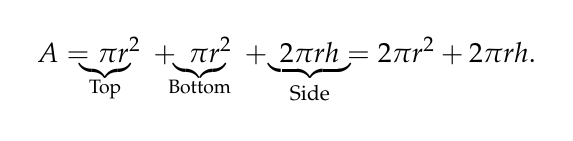
\begin{tikzpicture}[>=latex,name=myplot]
\draw  (2,2) node {$\displaystyle A= \pi r^2 ~+ ~\pi r^2~ + ~2\pi r h= 2\pi r^2 + 2\pi r h $.};
\draw (-.3,2) node [below] (a) {$\underbrace{\rule {0pt}{0pt}}$};
%\draw [->] (a) -- (.5,1);
\draw(-.3,1.75) node [below] {\scriptsize{Top}};

\draw (.9,2) node [below] (b) {$\underbrace{\rule {0pt}{0pt}}$};
\draw(.9,1.75) node [below] {\scriptsize{Bottom}};

\draw (2.3,2) node [below] (c) {$\underbrace{\rule {30pt}{0pt}}_{\scriptsize{\text{Side}}}$};
\end{tikzpicture}
\end{center}

Our surface area is now defined in terms of two variables. To reduce this to a single variable we use the volume of a can, $V=\pi r^2h$. Since the can must have $V= 8$ ft$^3$, we set $\pi r^2h=8$. Thus $\ds h =\frac{8}{\pi r^2}$ and \\
\begin{center} $A(r)=  2\pi r^2 + 2\pi r \frac{8}{\pi r^2} = 2\pi r^2 + \frac{16}{r}$ \end{center}

Next we find the critical values of $A(r)$. We compute $A'(r)$
\begin{center} $A'(r)=  4\pi r - \frac{16}{r^2}= \frac{4\pi r^3 - 16}{r^2}$ \end{center}

and solve $A'(r)=0$ 
\begin{center}$\ds r^3 = \frac{4}{\pi}$~~ or ~~$\ds r= \biggl(\frac {4}{\pi} \biggr)^{\frac{1}{3}} \approx 1.08$ ft. \end{center}

Looking back at $A(r)$ we notice that $r$ is not restricted to a closed interval. The radius can take on any positive value making the interval of optimization $(0, \infty)$. Since we do not have endpoints to test in $A(r)$ we consider what happens to $A(r)$ as $r$ approaches the enpoints of $(0, \infty)$. We see that \\ 
\begin{center}                          
$A(r) \to \infty$ as $r \to \infty$ (because of the $r^2$ term) and \vskip .25 truecm
$A(r) \to \infty$ as $r \to 0$ (because of the $\frac{16}{r}$ term)\\
\end{center} 
Thus, the surface area must minimized at the critical value, $\ds r= \biggl(\frac {4}{\pi} \biggr)^{\frac{1}{3}} \approx  $. Finally, we determine the height of the cylinder. \\

\begin{center} $h =\frac{8}{\pi r^2} =\frac{8}{\pi} r^{-2} = \frac{8}{\pi} \bigl((\frac {4}{\pi})^{\frac{1}{3}}\bigr)^{-2}=2(\frac{4}{\pi})(\frac {4}{\pi})^{-\frac{2}{3}}=2(\frac {4}{\pi})^{\frac{1}{3}}\approx 2.17$ ft.
 \end{center}

Notice that the height is twice the length of the radius. This means that the surface area is minimized when the can is as tall as it is wide.


\end{document}







